% Ejemplo de documento LaTeX
% Tipo de documento y tamaño de letra
\documentclass[12pt]{article}


\usepackage[spanish]{babel}
\usepackage{longtable} 
\selectlanguage{spanish}
\usepackage[utf8x]{inputenc}
\usepackage{graphicx}




% EL titulo, autor y fecha del documento
\title{Reporte de Actividad 5}
\author{Carlos Medina}
\date{03-03-15}


% Aqui comienza el cuerpo del documento
\begin{document}
% Construye el título
\maketitle


El siguiente reporte describirá los pasos realizados para la actividad 5 (2015-1), se explicarán y se mostrarán los resultados de ésta.




\hspace {0.5cm} El $Tiro$ $Parabolico$ es una forma de movimiento en el que un objeto o partícula (llamado proyectíl) es arrojado cerca de la superficie terrestre, y se mueve alrededor del trayecto de una curva bajo la acción de la gravedad sólamente. La única fuerza significante que actúa sobre el objeto es la gravedad, que actúa hacia abajo a causa de una aceleración hacia el centro de la Tierra. No hay fuerzas horizontales necesarias para mantener el movimiento horizontal – coherente con el concepto de inercia. 

El movimiento parabólico puede ser analizado como la composición de dos movimientos rectilíneos: un movimiento rectilíneo uniforme horizontal y un movimiento rectilíneo uniformemente acelerado vertical.
La trayectoria balística es la trayectoria de vuelo que sigue un proyectil sometido únicamente a su propia inercia y a las fuerzas inherentes al medio en el que se desplaza, principalmente la fuerza gravitatoria. La ciencia que estudia los fenómenos balísticos en general se denomina balística. La balistica exterior estudia la trayectoria balística bajo diversas condiciones.

Si el proyectil fue lanzado con una velocidad inicial $Vo$, entonces se puede describir con la expresión:

\begin{center}
	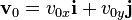
\includegraphics[width=3.5cm]{velin.png}\\
\end{center}

Los componentes $Vox$ y $Voy$ pueden ser encontrados si el angulo $0$ es conocido:

\begin{center}
	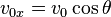
\includegraphics[width=3cm]{velx.png}\\
\end{center}
\begin{center}
	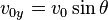
\includegraphics[width=3cm]{vely.png}\\
\end{center}

También se puede calcular el deslazamiento del cuerpo, definiéndose para el eje horizontal y vertical de la siguiente forma:


\begin{center}
	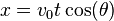
\includegraphics[width=3cm]{desx.png}\\
\end{center}
\begin{center}
	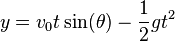
\includegraphics[width=4.5cm]{desy.png}\\
\end{center}

Con la información anterior, emezamos con las actividades.

Primeramente, se nos proporciona el siguiente código:

\begin{verbatim}

  program projectile_plot  
       implicit none  
       !Defining constants:  
       real, parameter :: pi = 4.0*atan(1.0) 
       real :: u, a, t, a_grados  
       real, parameter :: g = 9.81  
       real:: x(150),y(150)  
       integer :: i 

       !where g is gravity, pi is "pi"   
       !u is object's initial velocity   
       !a is object's initial angle   
       !t is time during the simulation   
       !x and y are arrays with 150 rows   
       !Seek user input   
       write(*,*) 'Enter angle of projectile (Real)'   
       read *, a_grados   
       write(*,*) 'Enter velocity of projectile (Real)'   
       read *, u   
       !Convert angle to radians   
       a = a_grados*pi/180.0   
       !open .dat file and start writing on it using the algorithm   
       open(1, file='proj.dat')   
         
       do i=1,100   
            !displacement of object in x and y direction   
            t = (float(i)*0.01)   
            x(i) = u*cos(a)*t   
            y(i) = u*sin(a)*t - 0.5*g*t*t   
            !write output in file "proj.dat" for plotting   
            write(1,*) x(i), y(i)   
            !kill the loop when the object hits the ground   
            if (y(i)<0) exit   
       end do   
       close(1)   
       !close file   
  end program projectile_plot 
\end{verbatim} 

Observamos que dentro del código, ha cambiado la salida standard a un archivo proj.dat, el cual posteriormente vas a graficar usando Gnuplot.  La parte del código que abre una unidad y escribe los datos se muestra abajo:

\begin{verbatim}
open (UNIT=1 , FILE=’proj.dat’) ! Open file 1 , call it proj.dat
 do i =1 ,imax ,1
      write (UNIT=1 ,*) x( i ) , y( i ) ! Write to proj .dat
 end do
close (UNIT=1) ! Close file 1 
\end{verbatim}

Con esto, se pide elaborar el programa de projectiles en Fortran 90, siguiendo el ejemplo brindado. Para esto, he cambiado el nombre de la salida "proj.dat" a "Tiro.dat", ya que me es más fácil ubicar el archivo.

Trataremos de reproducir resultados parecidos a los que muestra la simulación de Phet -una interfaz de simulaciónes proporcionadas por la Universidad de Colorado-, proporcionando la rapidez inicial y el ángulo de disparo, para encontrar la trayectoria del objeto y en que punto cae al suelo el proyectil.

También se nos pide incluir el cálculo del tiempo total de vuelo, la altura máxma que alcanza, y el alcance máximo del proyectil. Esto lo haremos de acuerdo a las ecuaciones de movimiento del tiro parabólico.

Modificamos las variables, agregando más variables, como el desplazamiento máximo en $x$ y en $y$. Usando estas variables, determinamos en el programa los pasos a realizar de acuerdo a las fórmulas, y nos quedó el siguiente código:

\begin{verbatim}
 program projectile_plot  
       implicit none  
       real, parameter :: pi = 4.0*atan(1.0) 
       real :: v, a, r, t, ym, xm, vx, vy
       real, dimension(1:3000) :: x,y 
       integer :: i 

       write(*,*) 'Ingresa el angulo inicial del proyectil en grados (Real)'   
       read *, a   
       write(*,*) 'Ingresa la velocidad inicial del proyectil en m/s (Real)'   
       read *, v   
       r = a*pi/180.0
     
       vx = (v)*(cos(r))
       vy = (v)*(sin(r))

       open(1, file='Tiro.dat')
       y = 0
       x = 0
       
       do i=1,3000  
            t = (float(i)*0.01)   
            x(i) = vx*t   
            y(i) = vy*t -4.9*t*t
     
            write(1,*) x(i), y(i)      
            if (y(i)<0) exit 
         
       end do

       close(1)   

       ym = (vy**2)/(19.6)
       xm = x(i)

       if (vx<0) then 
       xm = 0
       end if

       write(*,*) '°~~~~~°~~~~~°~~~~~°~~~~~°~~~~~°~~~~~°~~~~~~°~~~~~°~~~~~°~~~~~°~~~~~°~~~~~°'
       write(*,*) 'La altura maxima (y) es de: ', ym,'m'
       write(*,*) 'El tiempo total en el aire fue de:', t,'s'
       write(*,*) 'El alcance maximo (x) fue de:', xm,'m'
       write(*,*) 'Datos que usted ingreso:'
       write(*,*) 'Velocidad inicial:', v,'m/s'
       write(*,*) 'Angulo de tiro:', a,'° (', r,'radianes)'
       write(*,*) '°~~~~~°~~~~~°~~~~~°~~~~~°~~~~~°~~~~~°~~~~~~°~~~~~°~~~~~°~~~~~°~~~~~°~~~~~°'
  end program projectile_plot 
\end{verbatim}

Nótese que agregamos comandos para que nos diga cuál fue el resultado de cada cálculo.

Corremos el programa, y nos pedirá el ángulo y la velocidad inicial. Con la velocidad inicial de 5 m/s y el ángulo de 45°, nos salió el siguiente resultado:

\begin{center}
	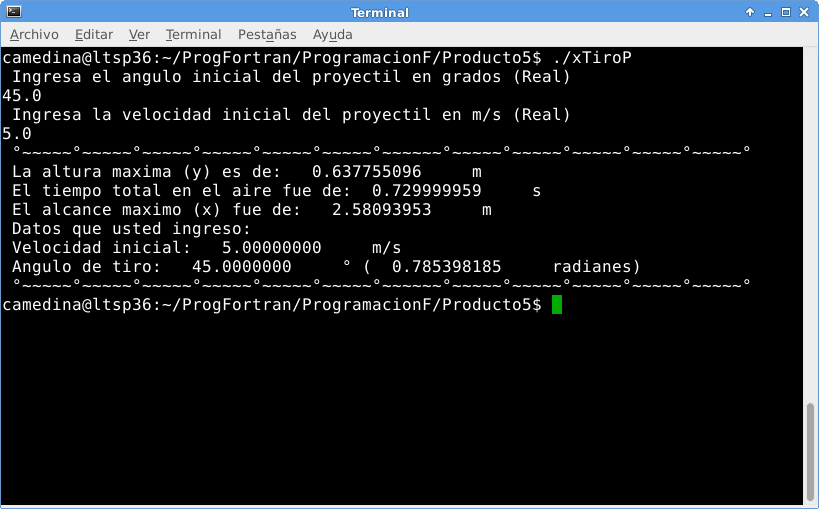
\includegraphics[width=14cm]{Resul.png}\\
\end{center}

Por último, abrimos $gnuplot$ en la terminal, graficamos el archivo, y nos resultó lo que esperábamos:


\begin{center}
	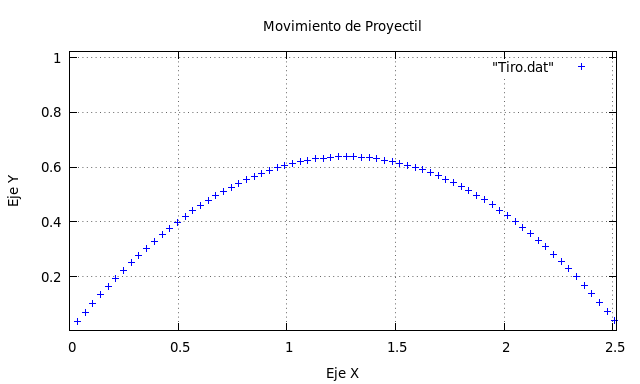
\includegraphics[width=15cm]{graf.png}\\
\end{center}

% Nunca debe faltar esta última linea.
\end{document}
